\documentclass[aspectratio=169]{beamer}

\usetheme{Boadilla}
\usefonttheme{professionalfonts}
\setbeamertemplate{navigation symbols}{}
\setbeamertemplate{itemize items}[circle]
\setbeamertemplate{enumerate items}[default]
\setbeamertemplate{headline}{}

\usepackage[utf8]{inputenc}
\usepackage[T1]{fontenc}
\usepackage{lmodern}
\usepackage{amsmath}
\usepackage{booktabs}
\usepackage{tabularx}
\usepackage{array}
\usepackage{hyperref}
\usepackage[strings]{underscore}
\usepackage{listings}
\usepackage{tikz}
\usetikzlibrary{arrows.meta,positioning,fit,calc,shapes.geometric}
\usepackage{xcolor}

\definecolor{courseblue}{HTML}{12355B}
\definecolor{coursegold}{HTML}{C98A2E}
\definecolor{courseice}{HTML}{EEF3F8}
\definecolor{coursegreen}{HTML}{2F6B4F}
\definecolor{coursegray}{HTML}{4B5563}
\definecolor{codebg}{HTML}{F7F9FC}
\definecolor{codecomment}{HTML}{5E6C84}
\definecolor{codestring}{HTML}{0B6E4F}

\setbeamercolor{palette primary}{bg=courseblue,fg=white}
\setbeamercolor{palette secondary}{bg=coursegold,fg=white}
\setbeamercolor{palette tertiary}{bg=courseblue,fg=white}
\setbeamercolor{palette quaternary}{bg=coursegold,fg=white}
\setbeamercolor{structure}{fg=courseblue}
\setbeamercolor{frametitle}{bg=courseice,fg=courseblue}
\setbeamercolor{title}{fg=courseblue}
\setbeamercolor{block title}{bg=courseblue,fg=white}
\setbeamercolor{block body}{bg=courseice,fg=black}
\setbeamercolor{normal text}{fg=black,bg=white}
\setbeamercolor{alerted text}{fg=coursegold}

\setbeamerfont{footline}{size=\scriptsize}

\setbeamertemplate{footline}{
  \leavevmode
  \hbox{
    \begin{beamercolorbox}[wd=.33\paperwidth,ht=2.8ex,dp=1.2ex,leftskip=0.8em]{palette primary}%
      University of Trieste
    \end{beamercolorbox}%
    \begin{beamercolorbox}[wd=.49\paperwidth,ht=2.8ex,dp=1.2ex,center]{palette tertiary}%
      \coursename{} \textbar{} \coursecode
    \end{beamercolorbox}%
    \begin{beamercolorbox}[wd=.18\paperwidth,ht=2.8ex,dp=1.2ex,rightskip=0.8em plus1fil]{palette secondary}%
      \insertframenumber{} / \inserttotalframenumber
    \end{beamercolorbox}%
  }
}

\hypersetup{
  colorlinks=true,
  linkcolor=courseblue,
  urlcolor=coursegreen
}

\lstdefinestyle{coursepython}{
  language=Python,
  basicstyle=\ttfamily\footnotesize,
  keywordstyle=\color{courseblue}\bfseries,
  commentstyle=\color{codecomment}\itshape,
  stringstyle=\color{codestring},
  showstringspaces=false,
  columns=fullflexible,
  keepspaces=true,
  frame=single,
  framerule=0.6pt,
  rulecolor=\color{courseblue},
  backgroundcolor=\color{codebg},
  xleftmargin=0.4em,
  xrightmargin=0.4em,
  aboveskip=0.4em,
  belowskip=0.2em
}

\newcommand{\coursename}{Data-driven Systems Engineering}
\newcommand{\coursecode}{440MI / 305SM}
\newcommand{\coursefooter}{}

\newcommand{\learninggoals}[1]{
  \begin{block}{Learning goals}
  #1
  \end{block}
}

\newcommand{\repoactivity}[1]{
  \begin{block}{Repo activity}
  #1
  \end{block}
}

\newcommand{\readinglist}[1]{
  \begin{block}{Papers and materials}
  {\footnotesize #1}
  \end{block}
}

\newcommand{\coursecontextframe}[5]{
  \begin{frame}{Course Map and Running Cases}
  \centering
  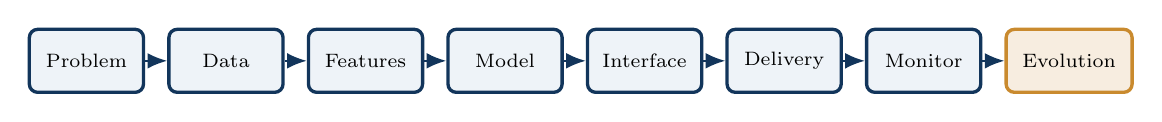
\begin{tikzpicture}[node distance=0.28cm]
  \node[flowbox, minimum width=1.45cm, minimum height=0.8cm] (problem) {\scriptsize Problem};
  \node[flowbox, minimum width=1.45cm, minimum height=0.8cm, right=of problem] (data) {\scriptsize Data};
  \node[flowbox, minimum width=1.45cm, minimum height=0.8cm, right=of data] (features) {\scriptsize Features};
  \node[flowbox, minimum width=1.45cm, minimum height=0.8cm, right=of features] (model) {\scriptsize Model};
  \node[flowbox, minimum width=1.45cm, minimum height=0.8cm, right=of model] (interface) {\scriptsize Interface};
  \node[flowbox, minimum width=1.45cm, minimum height=0.8cm, right=of interface] (delivery) {\scriptsize Delivery};
  \node[flowbox, minimum width=1.45cm, minimum height=0.8cm, right=of delivery] (monitor) {\scriptsize Monitor};
  \node[accentbox, minimum width=1.6cm, minimum height=0.8cm, right=of monitor] (evolution) {\scriptsize Evolution};
  \foreach \a/\b in {problem/data,data/features,features/model,model/interface,interface/delivery,delivery/monitor,monitor/evolution} {
    \draw[arrow] (\a) -- (\b);
  }
  \end{tikzpicture}

  \vspace{0.5em}
  \begin{block}{Today in the course}
  \textbf{Focus:} #1

  \textbf{Bridge:} #2
  \end{block}

  \begin{columns}[T]
  \column{0.48\textwidth}
  \begin{block}{Fraud case}
  {\footnotesize #3}
  \end{block}
  \column{0.48\textwidth}
  \begin{block}{Pasteurization case}
  {\footnotesize #4}
  \end{block}
  \end{columns}

  \vspace{0.3em}
  {\footnotesize \textbf{Course thread:} #5}
  \coursefooter
  \end{frame}
}

\newcommand{\classclosingframe}[4]{
  \begin{frame}{From This Class to the Next}
  \begin{block}{What stays with us}
  #1
  \end{block}

  \begin{columns}[T]
  \column{0.48\textwidth}
  \begin{block}{Project use}
  {\footnotesize #2}
  \end{block}
  \column{0.48\textwidth}
  \begin{block}{Next connection}
  {\footnotesize #3}
  \end{block}
  \end{columns}

  \vspace{0.3em}
  {\footnotesize \textbf{Course thread:} #4}
  \coursefooter
  \end{frame}
}

\tikzset{
  flowbox/.style={
    rounded corners=3pt,
    draw=courseblue,
    fill=courseice,
    very thick,
    minimum width=2.2cm,
    minimum height=0.9cm,
    align=center,
    font=\small
  },
  accentbox/.style={
    rounded corners=3pt,
    draw=coursegold,
    fill=coursegold!15,
    very thick,
    minimum width=2.2cm,
    minimum height=0.9cm,
    align=center,
    font=\small
  },
  arrow/.style={
    -{Latex[length=2.5mm,width=2mm]},
    thick,
    draw=courseblue
  }
}


\title{Class 11: Python --- First Contact with the scikit-learn API}
\author{\coursename}
\date{}

\begin{document}

\frame{\titlepage \coursefooter}

\begin{frame}{Agenda}
\begin{itemize}
\item The scikit-learn contract: \texttt{fit}, \texttt{predict}, and why every estimator shares it.
\item Splitting data with \texttt{train\_test\_split}.
\item Training an estimator, and searching over one with \texttt{GridSearchCV}.
\item The Pipeline pattern for chaining steps.
\item What this class deliberately leaves for the Data-Driven block.
\end{itemize}
\coursefooter
\end{frame}

\begin{frame}{Learning goals}
\learninggoals{
\begin{itemize}
\item Call \texttt{train\_test\_split} correctly and explain its main arguments.
\item Instantiate a scikit-learn estimator and call \texttt{.fit()} and \texttt{.predict()} on it.
\item Recognize \texttt{GridSearchCV} as an object with the same \texttt{fit} contract as any estimator.
\item Describe what a \texttt{Pipeline} chains together and why.
\item State clearly which questions are programming mechanics today, and which are modeling theory for later.
\end{itemize}
}
\coursefooter
\end{frame}

\coursecontextframe
{The scikit-learn API as programming mechanics: fit, predict, and pipeline, not model theory.}
{Class 8 showed that \texttt{RandomForestClassifier} and \texttt{StandardScaler} are just classes; today is about the shared calling convention every scikit-learn class honors.}
{The fraud model in `streamlit/modeling.py` is trained with exactly the same three calls this class walks through: split, fit, predict.}
{The pasteurization case will eventually reuse the same estimator contract for a forecasting or anomaly-detection model, whatever the algorithm turns out to be.}
{Learn the shape of the API once, and the same four or five method calls carry you through almost any scikit-learn model this course uses.}

\begin{frame}{The scikit-learn contract}
\begin{itemize}
\item Every estimator is instantiated the same way: \texttt{Estimator(hyperparameters)}.
\item Every estimator is trained the same way: \texttt{estimator.fit(X, y)}.
\item Every estimator predicts the same way: \texttt{estimator.predict(X)}.
\item This uniform contract is a deliberate design choice, not an accident --- it is what let Class 8's inheritance discussion matter in practice.
\end{itemize}
\begin{block}{Why it matters}
Once you can call \texttt{.fit()} and \texttt{.predict()} on one estimator, you can call it on almost any other, without relearning an API.
\end{block}
\coursefooter
\end{frame}

\begin{frame}[fragile]{Loading data and splitting it}
\begin{lstlisting}[style=coursepython]
iris = load_iris()
X = pd.DataFrame(iris.data, columns=iris.feature_names)
y = pd.Series(iris.target, name='target')

X_train, X_test, y_train, y_test = train_test_split(
    X, y, test_size=0.3, random_state=42, stratify=y
)
\end{lstlisting}
\begin{itemize}
\item From `notebooks/Class6\_Model\_Training\_.ipynb`: one function call turns one dataset into four pieces.
\item This is pure mechanics --- \emph{why} we split before training is a modeling-theory question for the Data-Driven block.
\end{itemize}
\coursefooter
\end{frame}

\begin{frame}{What \texttt{train\_test\_split}'s arguments do}
\begin{tabularx}{\textwidth}{>{\bfseries}l X}
Argument & Mechanical effect \\
\toprule
\texttt{test\_size} & Fraction of rows set aside as \texttt{X\_test}/\texttt{y\_test}. \\
\texttt{random\_state} & Fixes the random shuffle so the split is reproducible. \\
\texttt{stratify} & Splits so each subset keeps the same class proportions as \texttt{y}. \\
\bottomrule
\end{tabularx}
\vspace{0.4em}
\begin{itemize}
\item Notice all three arguments only control \emph{how the split happens}, not whether it is the right thing to do --- that judgment call belongs to a later class.
\end{itemize}
\coursefooter
\end{frame}

\begin{frame}[fragile]{Instantiate, then fit}
\begin{lstlisting}[style=coursepython]
rf = RandomForestClassifier(random_state=42)
rf.fit(X_train, y_train)
y_pred = rf.predict(X_test)
\end{lstlisting}
\begin{itemize}
\item Three lines: build the object, train it in place, ask it for predictions on unseen rows.
\item `streamlit/modeling.py` follows the identical shape with a scaler in between: \texttt{scaler.fit\_transform(X\_train)} then \texttt{cls.fit(X\_train\_scaled, y\_train)}.
\end{itemize}
\coursefooter
\end{frame}

\begin{frame}[fragile]{\texttt{GridSearchCV}: still just \texttt{.fit()}}
\begin{lstlisting}[style=coursepython]
param_grid = {
    'n_estimators': [50, 100, 200],
    'max_depth': [3, 5, 8, None],
    'min_samples_split': [2, 4, 6]
}

grid = GridSearchCV(rf, param_grid, cv=5, scoring='accuracy', n_jobs=-1)
grid.fit(X_train, y_train)
\end{lstlisting}
\begin{itemize}
\item From the same notebook: \texttt{GridSearchCV} wraps an estimator and a grid of hyperparameters, but is itself called with \texttt{.fit()}, exactly like \texttt{rf} above.
\item What \texttt{cv} and \texttt{scoring} actually optimize for is a modeling-theory question we postpone; today, notice only that the calling convention never changes.
\end{itemize}
\coursefooter
\end{frame}

\begin{frame}[fragile]{What comes back out}
\begin{lstlisting}[style=coursepython]
grid.best_params_
grid.best_score_
best_model = grid.best_estimator_

y_pred = best_model.predict(X_test)
\end{lstlisting}
\begin{itemize}
\item After \texttt{.fit()}, \texttt{grid} carries fitted attributes: the winning parameters, its score, and the trained estimator itself.
\item \texttt{best\_model} is just another estimator --- \texttt{.predict()} works on it exactly as it did on \texttt{rf}.
\end{itemize}
\coursefooter
\end{frame}

\begin{frame}[fragile]{The Pipeline pattern}
\begin{lstlisting}[style=coursepython]
from sklearn.pipeline import Pipeline

pipe = Pipeline([
    ("scaler", StandardScaler()),
    ("model", RandomForestClassifier(random_state=42)),
])
pipe.fit(X_train, y_train)
pipe.predict(X_test)
\end{lstlisting}
\begin{itemize}
\item This is the idiomatic scikit-learn way to chain the scaler and the model into one object --- not yet how `modeling.py` is written, which fits the scaler and the model as two separate steps.
\item A \texttt{Pipeline} is itself an estimator: it honors the same \texttt{.fit()} / \texttt{.predict()} contract as its individual pieces.
\end{itemize}
\coursefooter
\end{frame}

\begin{frame}{Why the uniform API is worth learning on purpose}
\begin{itemize}
\item Swapping \texttt{RandomForestClassifier} for a different classifier changes one line, not the surrounding pipeline.
\item A \texttt{GridSearchCV}-wrapped estimator, or a \texttt{Pipeline}-wrapped one, both still expose \texttt{.fit()} and \texttt{.predict()}.
\item This is Class 8's inheritance discussion paying off directly: shared base classes are what make this consistency possible.
\end{itemize}
\coursefooter
\end{frame}

\begin{frame}{What today deliberately does not cover}
\begin{itemize}
\item Why accuracy can mislead on an imbalanced target like fraud detection.
\item How to choose \texttt{cv}, \texttt{scoring}, or a hyperparameter grid.
\item Feature scaling and encoding theory --- only the mechanical call, \texttt{.fit\_transform()}, was shown.
\item All of the above belong to the Data-Driven block, once the programming mechanics here are second nature.
\end{itemize}
\coursefooter
\end{frame}

\begin{frame}{How the repo already uses today's building blocks}
\repoactivity{
\begin{itemize}
\item `notebooks/Class6\_Model\_Training\_.ipynb` runs \texttt{train\_test\_split}, a plain \texttt{RandomForestClassifier}, and a \texttt{GridSearchCV} over it, in that order.
\item `streamlit/modeling.py` shows the two-step, non-Pipeline version of scaling and fitting.
\item Rewrite `modeling.py`'s scaler-then-classifier steps as a single \texttt{Pipeline} and check that \texttt{.predict()} still works.
\end{itemize}
}
\coursefooter
\end{frame}

\begin{frame}{Discussion prompt}
\begin{block}{Question}
`GridSearchCV` and `Pipeline` both wrap other estimators, yet both expose the same \texttt{.fit()} / \texttt{.predict()} interface as a plain classifier. What design principle from Class 8 makes that possible?
\end{block}
\begin{itemize}
\item Ties directly back to inheritance and shared base classes, rather than treating the API's consistency as a coincidence.
\end{itemize}
\coursefooter
\end{frame}

\begin{frame}{Papers and materials}
\readinglist{
\href{https://arxiv.org/abs/1309.0238}{Buitinck et al.\ (2013), API design for machine learning software};\
\href{https://www.jmlr.org/papers/volume12/pedregosa11a/pedregosa11a.pdf}{Pedregosa et al.\ (2011), scikit-learn: Machine Learning in Python};\
\href{https://scikit-learn.org/stable/modules/compose.html}{scikit-learn pipelines and composite estimators};\
\href{https://scikit-learn.org/stable/modules/generated/sklearn.model_selection.GridSearchCV.html}{GridSearchCV API}.
}
\coursefooter
\end{frame}

\classclosingframe
{\begin{itemize}
\item \texttt{fit}, \texttt{predict}, and the constructor call are the three moves that carry you through almost any scikit-learn estimator.
\item \texttt{GridSearchCV} and \texttt{Pipeline} are themselves estimators --- the API does not change as objects wrap other objects.
\item Metrics, scoring choices, and hyperparameter theory are intentionally still ahead of us.
\end{itemize}}
{Any project step described as ``train a scikit-learn model'' is exactly today's three-call shape, whatever the model turns out to be.}
{Class 12 is a guided lab: applying this course's full EDA workflow to a fresh dataset, hands-on.}
{Mechanics without practice fade fast --- the next session is where you drive.}

\end{document}
